\paragraph{Représentation graphique des CU}
%~\par
Les CU peuvent être représentés sous forme graphique, voir la figure \ref{schema_diag_cu} pour un exemple. Les acteurs directs sont représentés sous forme de petits personnages. Dans les bulles, sont représentés les cas d'utilisation. Un trait entre un acteur et un CU indique que l'acteur participe à ce CU. Les liens hachurés entre CU, étiquetés par le mot <<use>> (ou <<include>>), indiquent que ce CU fait appel à l'autre CU --- on parle alors de sous-cas d'utilisation. Les liens hachurés entre CU, étiquetés par le mot <<extend>>, indique qu'il s'agit d'une extension d'un CU : un CU qui ne se déclenche que sous certaines conditions.

\begin{minipage}{1\linewidth} 
    \centering
    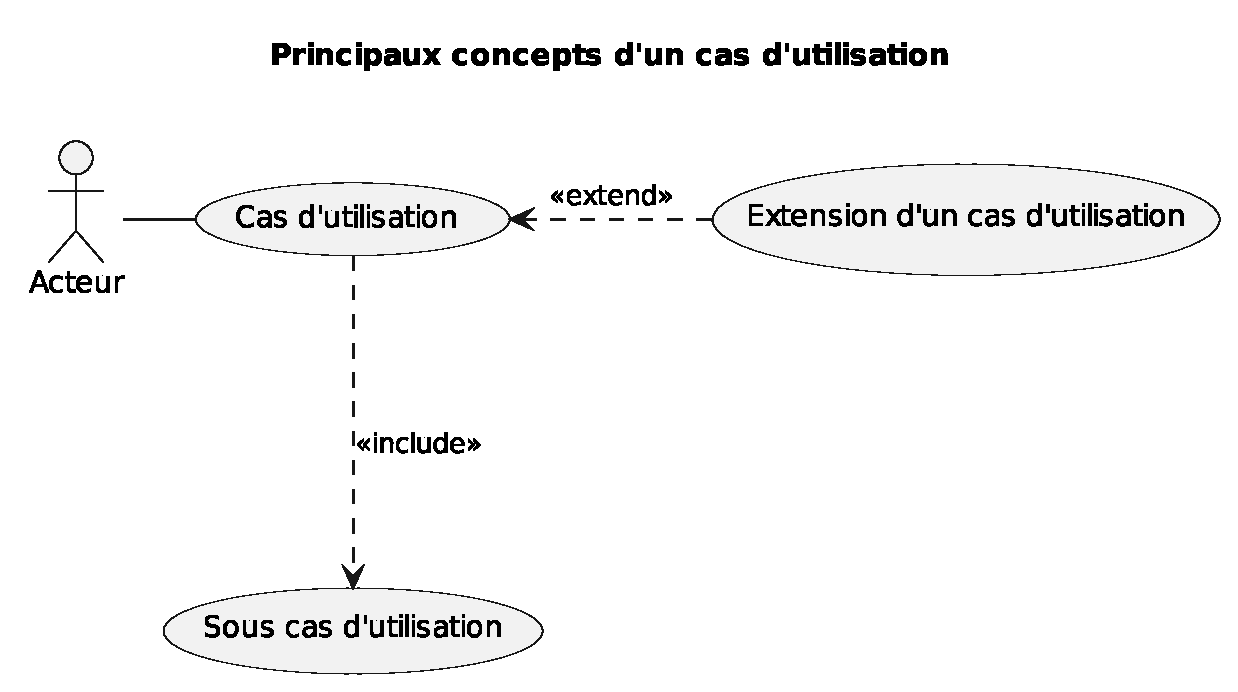
\includegraphics[width=14cm]{../schemas/exemple_diag_cu}
    \captionsetup{justification=centering}
    \captionof{figure}{Légende explicative d'un diagamme de cas d'utilisation UML}
    \label{schema_diag_cu}
\end{minipage}

\paragraph{Représentation textuelle des CU}
%~\par
La description textuelle des cas d'utilisation est souvent présentée sous forme d'un tableau constitué de champs suivants : 
\begin{longtable}[l]{|p{3cm}|p{11.7cm}|}
    \hline
        Titre & Rappelle en quelques mots l'objectif principal du cas d'utilisation.\\
    \hline
        Résumé & Décrit brièvement le comportement du cas d'utilisation.\\
    \hline
        Portée & Définit la portée de conception du CU (étendue spatiale).\\
    \hline
        Niveau & Niveau de granularité du cas d'utilisation (stratégique, utilisateur ou sous-fonction).\\
    \hline
        Acteurs directs & Acteurs qui participent au CU.\\
    \hline 
        Acteurs indirects & Acteurs qui ne participent pas au CU, mais qui ont un intérêt dans sa réalisation.\\
    \hline
        Préconditions & Ensemble des conditions qui doivent être vérifiées avant le déroulement du CU. Les
        préconditions, sans mention contraire explicite, des CU parents au CU doivent
        toujours être vérifiées.\\
    \hline
        Garanties \newline minimales & Définissent ce qui est garanti par le système à l'étude même en cas d'échec du cas d'utilisation.\\
    \hline
        Garanties en cas de succès & Définissent les garanties en cas de succès (par le scénario nominal ou par ses
        variantes). \\
    \hline
        Scénario nominal & C'est un scénario représentatif de l'utilisation du système où tout se passe bien. Il
        se termine par la réussite des objectifs. Il peut être constitué d'une condition
        déclenchant le scénario, d'un ensemble d'étapes, d'une condition de fin, et
        éventuellement d'extensions ou de variantes. Une étape peut être une interaction
        entre acteurs, une étape de validation, ou un changement interne.\\
    \hline
        Variantes & Lorsqu'il y a plusieurs façons de procéder à une même étape sans remise en cause
        du scénario nominal.\\
    \hline
        Extensions & Définissent les autres scénarios que le scénario nominal (par exemple ceux qui se
        terminent par un échec). Ils se déclenchent sur des conditions spécifiques
        détectées par le SàE.\\
    \hline
        Informations \newline complémentaires & Informations diverses nécessaires à la compréhension du CU. \\
    \hline
\end{longtable}